\documentclass[a4paper]{article}

\usepackage[spanish]{babel}
	\selectlanguage{spanish}
\usepackage{geometry}
	\newgeometry{margin=3cm}
\usepackage{setspace}
\usepackage{graphicx}
\usepackage{float}
\usepackage[utf8]{inputenc}

\title{Reporte del Producto 4}
\author{Ana Gabriela Carretas Talamante}
\date{09 de marzo de 2015}

\begin{document}
\maketitle
\section{¿Qué es un Polinomio de Taylor?}
Antes de abordar la relación que hay entre "Taylor" y los polinomios, tendremos que escrutar los orígenes de esta útil herramienta, misma que precede al cálculo integral. \\ \\
Sabemos que la recta tangente, como la mejor aproximación lineal a la gráfica de f en las cercanías del punto de tangencia $(x_o, f(x_o))$, es aquella recta que pasa por el mencionado punto y tiene la misma pendiente que la curva en ese punto (primera derivada en el punto), lo que hace que la recta tangente y la curva sean prácticamente indistinguibles en las cercanías del punto de tangencia. \\ \\
  
Veamos qué sucede si en lugar de aproximarnos con una recta, tratamos de hacerlo con una parábola, es decir, tratemos de encontrar \textit{"la parábola tangente"}.

\begin{figure}[H]
    \centering
    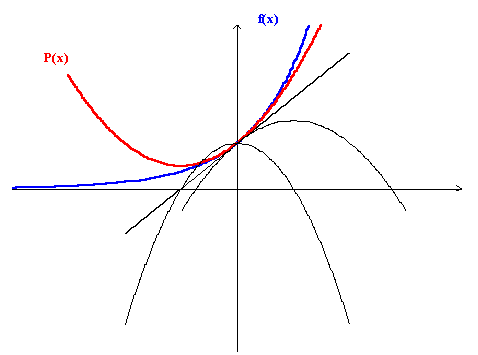
\includegraphics[width=12cm]{1}
  \end{figure} 

Naturalmente a esta parábola $f(P) = a + b(x- x_o) + c(x- x_o)$ debemos pedirle que pase por el punto, que tenga la misma inclinación (primera derivada) y la misma concavidad que la parábola (segunda derivada), es decir debemos pedirle:

\begin{itemize}
\item $P(x_o)=f(x_o)$
\item $P'(x_o)=f'(x_o)$
\item $P''(x_o)=f''(x_o)$
\end{itemize}

quedando la ecuación de la parábola que mejor aproxima a la curva en las cercanías de $(x_o,f(x_o))$, como: $$f(x_o)=f(x_o)+f'(x_o)(x-x_o)+\frac{f''(x_o)}{2}(x-x_o)$$
  \begin{figure}
    \centering
    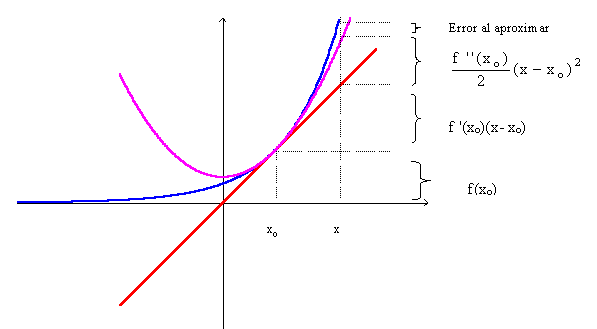
\includegraphics[width=12cm]{2}
    \caption{Ecuación de $P(x)$ gráficamente}
  \end{figure}

Dado un polinomio cualquiera podemos expresarlo en potencias de $(x-x_0)$ para cualquier $x_o$. Sus coeficientes estarán en función de las derivadas en $x_o$. Asimismo, si conocemos las derivadas en un punto $x_o$, podemos encontrar un polinomio de grado $n$ que satisfaga la mejor aproximación a la función. Obteniendo entonces un \textbf{Polinomio de Taylor de grado $n$ para $f$, en el punto $x_o$} de esta manera:
$$P_n(x)=f(x_o)+f'(x_o)(x-x_o)+\frac{f^{(2)}(x_o)}{2}(x-x_o)^2+\ddots+\frac{f^{(n)}(x_o)}{n}(x-x_o)^n$$

Esta aproximación tiene tres ventajas importantes:
\begin{itemize}
\item La derivación e integración de una de estas series se puede realizar término a término, y resultan operaciones triviales.
\item Se puede utilizar para calcular valores aproximados de funciones.
\item Es posible calcular la optimidad de la aproximación.
\end{itemize}

\section{Graficando funciones en \texttt{Maxima}}
  \subsection{Polinomios de Taylor para $\sin(x)$}
  \label{1}
    Se pidió que graficáramos la aproximación de Taylor para $\sin(x)$.
    
    \subparagraph{Código en \texttt{Maxima}}
      \begin{verbatim}
      f(x):=sin(x);
      T1(x):=taylor(f(x), x, 0, 1);
      T3(x):=taylor(f(x), x, 0, 3);
      T5(x):=taylor(f(x), x, 0, 5);
      T7(x):=taylor(f(x), x, 0, 7);
      fortran(T1(x));
      fortran(T3(x));
      fortran(T5(x));
      fortran(T7(x));
      text(T1(x));
      text(T3(x));
      text(T5(x));
      text(T7(x));
      plot2d ([f(x),T1(x),T3(x),T5(x),T7(x)],[x, -3.5, 3.5], [y, -1.5, 1.5,
      [grid2d,true],[color,red,green,blue,orange,gray],[legend,false],
      [label,["y=sin(x)",3,0.2],["y=P1(x)",1.5,1.5],["y=P3(x)",2.3,-1],
      ["y=P5(x)",3,0.85],["y=P7(x)",3,-0.65]],[axes, solid],[box,false],
      [xlabel,"x"], [ylabel,"y"]);
      \end{verbatim}
      
      \begin{figure}[H]
        \centering
        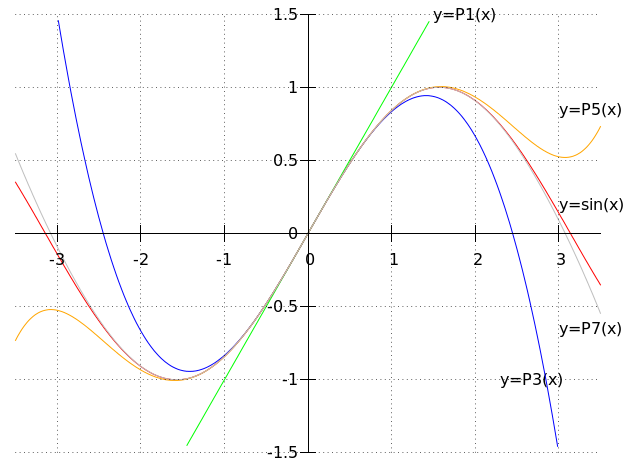
\includegraphics[width=12cm]{sen_x}
        \caption{Gráfica de \ref{1} en \texttt{gnuplot}}
      \end{figure}

  \subsection{Polinomios de Taylor para $log(1+x)$}
  \label{2}
  	Se pidió que graficáramos la aproximación de Taylor para $log(1+x)$.
  
  	\subparagraph{Código en \texttt{Maxima}}
      \begin{verbatim}
      T4(x):=taylor(f(x), x, 0, 4);
      T7(x):=taylor(f(x), x, 0, 7);
      T11(x):=taylor(f(x), x, 0, 11);
      T16(x):=taylor(f(x), x, 0, 16);
      f(x):=log(1+x);
      fortran(T4(x));
      fortran(T7(x));
      fortran(T11(x));
      fortran(T16(x));
      text(T4(x));
      text(T7(x));
      text(T11(x));
      text(T16(x));
      plot2d ([T4(x),T7(x),T11(x),T16(x),f(x)], [x, -1.5, 1.5], [y, -4, 2],
      [grid2d,true],[axes,solid],[color,red,green,blue,cyan,orange], 
      [legend,"T4","T7","T11","T16","log(1+x)"],[gnuplot_preamble, "set key left"]);
      \end{verbatim}
  
      \begin{figure}[H]
        \centering
        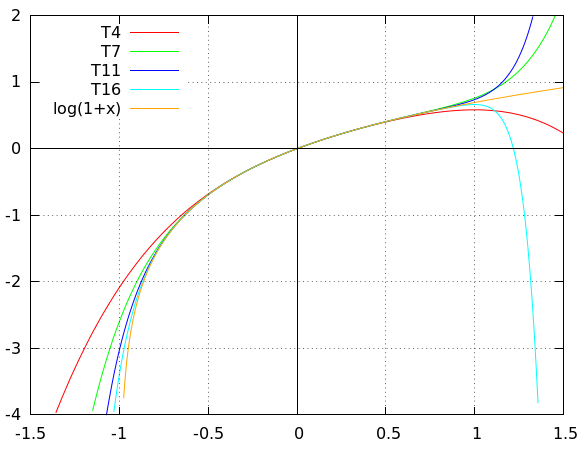
\includegraphics[width=12cm]{log_1+x}
        \caption{Gráfica de \ref{2} en \texttt{gnuplot}}
      \end{figure}
    
  \subsection{Polinomios de Taylor para $log(cos(x))$}
  \label{3}
  	También se presenta la gráfica para $log(cos(x))$.
    
    \subparagraph{Código con \texttt{Maxima}}
      \begin{verbatim}
      T3(x):=taylor(f(x), x, 0, 3);
      T5(x):=taylor(f(x), x, 0, 5);
      T7(x):=taylor(f(x), x, 0, 7);
      T9(x):=taylor(f(x), x, 0, 9);
      f(x):=log(cos(x));
      fortran(T3(x));
      fortran(T5(x));
      fortran(T7(x));
      fortran(T9(x));
      text(T3(x));
      text(T5(x));
      text(T7(x));
      text(T9(x));
      plot2d ([T3(x),T5(x),T7(x),T9(x),f(x)], [x, -%pi/2, %pi/2], [y, -6, 2],
      [grid2d,true],[axes,solid],[color,red,green,blue,cyan,orange], 
      [legend,"T3","T5","T7","T9","log(cos(x))"],[xlabel,"x"],[ylabel, "y"]);
      \end{verbatim}
    
      \begin{figure}[H]
        \centering
        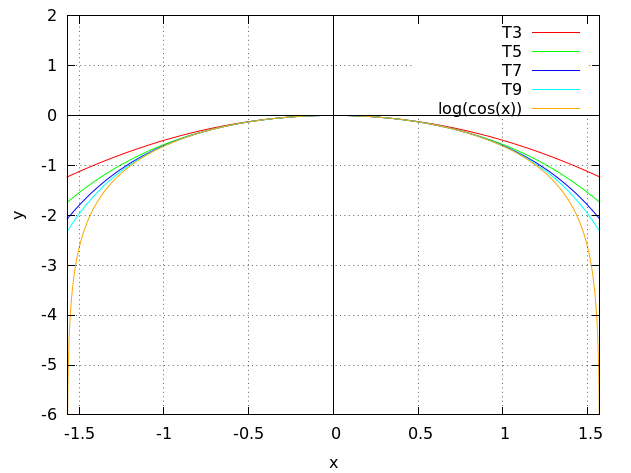
\includegraphics[width=12cm]{log_cosx}
        \caption{Gráfica de \ref{3} en \texttt{gnuplot}}
      \end{figure}
      
  \subsection{Polinomios de Taylor para $\frac{e ^{x}}{\cos(x)}$}
  \label{4}
  	Se obtuvieron resultados de $\frac{e^{x}}{\cos(x)}$ en las cercanías del $0$.
    
    \subparagraph{Código con \texttt{Maxima}}
      \begin{verbatim}
      T3(x):=taylor(f(x), x, 0, 3);
      T5(x):=taylor(f(x), x, 0, 5);
      T7(x):=taylor(f(x), x, 0, 7);
      T9(x):=taylor(f(x), x, 0, 9);
      f(x):=exp(x)/cos(x);
      fortran(T3(x));
      fortran(T5(x));
      fortran(T7(x));
      fortran(T9(x));
      text(T3(x));
      text(T5(x));
      text(T7(x));
      text(T9(x));
      plot2d ([T3(x),T5(x),T7(x),T9(x),f(x)], [x, -%pi, %pi], [y, -5, 5,
      [grid2d,true],[axes,solid],[color,red,green,blue,cyan,orange], 
      [legend,"T3","T5","T7","T9","exp(x)/cos(x)"],[xlabel,"x"],[ylabel, "y"]);
      \end{verbatim}
 
      \begin{figure}[H]
        \centering
        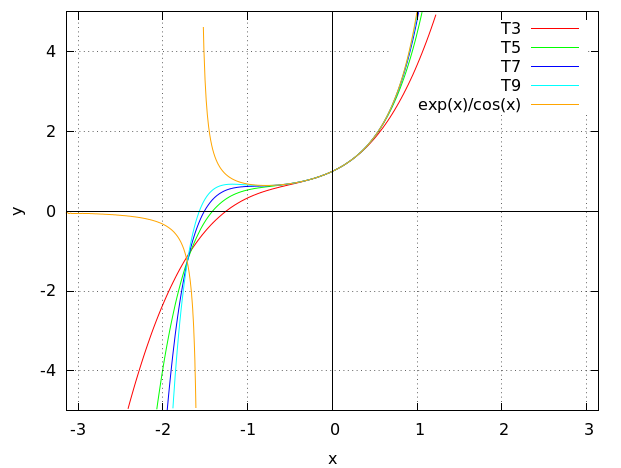
\includegraphics[width=12cm]{expx_cosx}
        \caption{Gráfica de \ref{4} en \texttt{gnuplot}}
      \end{figure}

  \subsection{Polinomios de Taylor para $(1+x)(e^x)$}
  \label{5}
  	Por último, tenemos la aproximación de $(1+x)(e^x)$.
    
    \subparagraph{Código con \texttt{Maxima}}
      \begin{verbatim}
      T3(x):=taylor(f(x), x, 0, 3);
      T5(x):=taylor(f(x), x, 0, 5);
      T7(x):=taylor(f(x), x, 0, 7);
      T9(x):=taylor(f(x), x, 0, 9);
      f(x):=(1+x)*(exp(x));
      fortran(T3(x));
      fortran(T5(x));
      fortran(T7(x));
      fortran(T9(x));
      text(T3(x));
      text(T5(x));
      text(T7(x));
      text(T9(x));
      plot2d ([T3(x),T5(x),T7(x),T9(x),f(x)], [x, -5, 2], [y, -5, 5],[grid2d,true],
      [axes,solid],[color,red,green,blue,cyan,orange], 
      [gnuplot_preamble, "set key left"], 
      [legend,"T3","T5","T7","T9","(1+x)*(exp(x))"],[xlabel,"x"],[ylabel, "y"]);
            \end{verbatim}
    
      \begin{figure}[H]
        \centering
        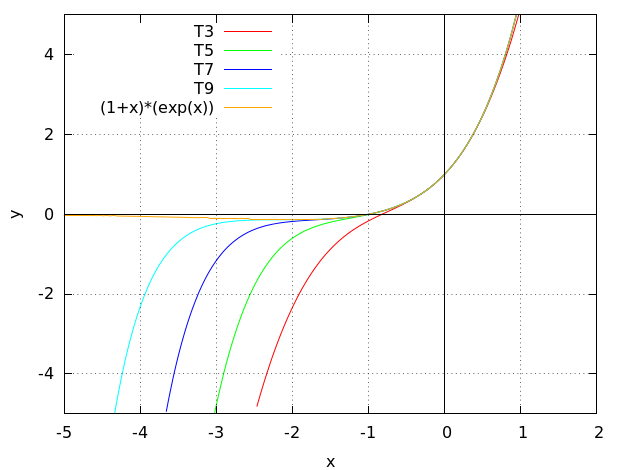
\includegraphics[width=12cm]{1+x_expx}
        \caption{Gráfica de \ref{5} en \texttt{gnuplot}}
      \end{figure}
      
\end{document}